% Definiere eine Funktion zum Zeichnen eines Rechtecks
\newcommand{\drawRectangle}[4]{
	\def\xcenter{#1} % x-Koordinate des Mittelpunkts
	\def\ycenter{#2} % y-Koordinate des Mittelpunkts
	\def\width{#3}   % Breite des Rechtecks
	\def\height{#4}  % Höhe des Rechtecks
	
	% Berechne die Ecken des Rechtecks
	\def\xmin{\xcenter - \width/2}
	\def\xmax{\xcenter + \width/2}
	\def\ymin{\ycenter - \height/2}
	\def\ymax{\ycenter + \height/2}
	
	% Zeichne das Rechteck
	\fill[orange] (\xmin, \ymin) rectangle (\xmax, \ymax);
}

\setlength{\unitlength}{0.1mm}
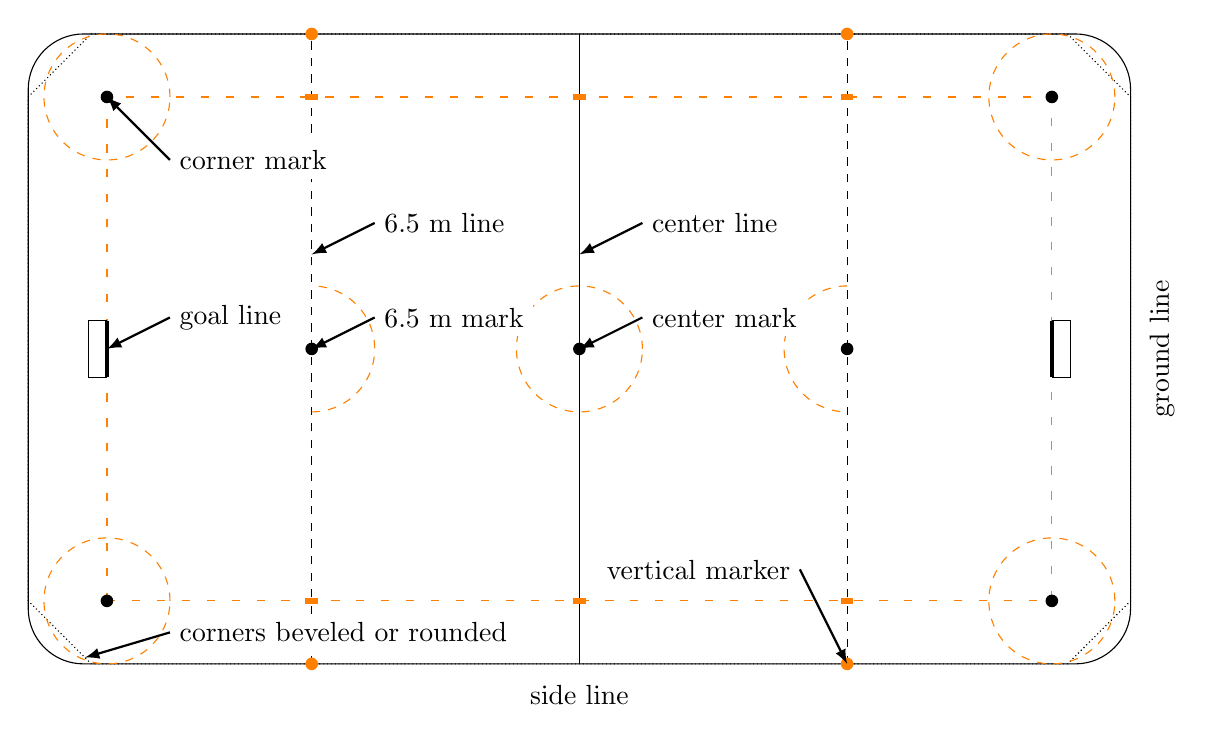
\begin{tikzpicture}[scale=0.4]%(1600,1000)
\usetikzlibrary{calc}
% length:
\dimline[line style = {line width=0.9},]{(0,21)}{(35,21)}{length: 35 - 45 m}
\dimline[line style = {line width=0.9},]{(-1,0)}{(-1,20)}{breadth: 20 - 25 m}
\dimline[line style = {line width=0.9},]{(35-2.5-6.5,15)}{(35-2.5,15)}{6.5 m}
\dimline[label style={above=0.5ex,}, line style = {line width=0.9},]{(32.5,5)}{(35,5)}{2.5 m}
\dimline[label style={above=0.5ex,}, line style = {line width=0.9},]{(28.75,0)}{(28.75,2)}{2 m}

% field:
\draw[rounded corners=20pt] (0,0) rectangle ++(35,20);
\draw[densely dotted] (0,2) -- (0,18) -- (2,20) -- (33,20) -- (35,18) -- (35,2) -- (33,0) -- (2,0) -- (0,2);
\draw[orange, loosely dashed] (2.5,2) -- (2.5,18) -- (32.5,18) -- (32.5,2) -- (2.5,2);
% corner marks:
\fill (2.5,2) circle (0.2);
\draw[orange, dashed] (2.5,2) circle (2);
\fill (2.5,18) circle (0.2);
\draw[orange, dashed] (2.5,18) circle (2);
\fill (35-2.5,18) circle (0.2);
\draw[orange, dashed] (35-2.5,18) circle (2);
\fill (35-2.5,2) circle (0.2);
\draw[orange, dashed] (35-2.5,2) circle (2);
% center line:
\draw[] (17.5,0) -- (17.5,20);
% center mark:
\fill (17.5,10) circle (0.2);
\draw[orange, dashed] (17.5,10) circle (2);
% 6.5 m lines:
\draw[dashed] (2.5+6.5,0) -- (2.5+6.5,20);
\draw[dashed] (35-2.5-6.5,0) -- (35-2.5-6.5,20);
% 6.5 m marks:
\fill (2.5+6.5,10) circle (0.2);
\draw[orange, dashed] (2.5+6.5,8) arc(-90:90:2);
\fill (35-2.5-6.5,10) circle (0.2);
\draw[orange, dashed] (35-2.5-6.5,12) arc(90:270:2);
% goal line:
\draw[line width=0.5mm,] (2.5,9.1) -- (2.5,10.9);
\draw[line width=0.5mm,] (35-2.5,9.1) -- (35-2.5,10.9);

%intersection marks:
%\fill[orange] (2.5+6.5,2) circle (0.2);
%\fill[orange] (2.5+6.5,18) circle (0.2);
%\fill[orange] (17.5,2) circle (0.2);
%\fill[orange] (17.5,18) circle (0.2);
%\fill[orange] (35-2.5-6.5,2) circle (0.2);
%\fill[orange] (35-2.5-6.5,18) circle (0.2);
\drawRectangle{2.5+6.5}{2}{0.4}{0.2}
\drawRectangle{2.5+6.5}{18}{0.4}{0.2}
\drawRectangle{17.5}{2}{0.4}{0.2}
\drawRectangle{17.5}{18}{0.4}{0.2}
\drawRectangle{35-2.5-6.5}{2}{0.4}{0.2}
\drawRectangle{35-2.5-6.5}{18}{0.4}{0.2}

%vertival marks
\fill[orange] (2.5+6.5,0) circle (0.2);
\fill[orange] (2.5+6.5,20) circle (0.2);
\fill[orange] (35-2.5-6.5,0) circle (0.2);
\fill[orange] (35-2.5-6.5,20) circle (0.2);

% goals
\draw (2.5,9.1) -- (1.9,9.1) -- (1.9,10.9) -- (2.5,10.9);
\draw (32.5,9.1) -- (33.1,9.1) -- (33.1,10.9) -- (32.5,10.9);

% labels
\node[right, fill=white] at (4.5,16) (Corner-Mark) {corner mark};
\draw[-latex,thick] (4.5,16) -- (2.5,18);
\node[right] at (4.5,11) (Goal-Line) {goal line};
\draw[-latex,thick] (4.5,11) -- (2.5,10);
\dimline[line style = {line width=0.9},]{(0,5)}{(2.5+6.5,5)}{goal area}
%\node[fill=white] at (4.75,5) (Goal-Area) {goal area};
\node[right, fill=white] at (11,11) (6.5-Mark) {6.5 m mark};
\draw[-latex,thick] (11,11) -- (2.5+6.5,10);
\node[right] at (11,14) (6.5-Line) {6.5 m line};
\draw[-latex,thick] (11,14) -- (2.5+6.5,13);
\node[right, fill=white] at (19.5,11) (Center-Mark) {center mark};
\draw[-latex,thick] (19.5,11) -- (17.5,10);
\node[right] at (19.5,14) (Center-Line) {center line};
\draw[-latex,thick] (19.5,14) -- (17.5,13);
\node[left, fill=white] at (24.5,3) (VerticalMarker) {vertical marker};
\draw[-latex,thick] (24.5,3) -- (26,0);
\node at (17.5,-1) (Side-Line) {side line};
\node[rotate=90] at (36,10) (Ground-Line) {ground line};

\node[right, fill=white] at (4.5,1) {corners beveled or rounded};
\draw[-latex,thick] (4.5,1) -- (1.8,0.2);
\end{tikzpicture}
